% 1.6 Phương pháp hình học
\begin{frame}{1.6 PHƯƠNG PHÁP HÌNH HỌC
\hspace{3cm}  70. Nguyễn Phương Thùy} 
%\framesubtitle{} 
\begin{block}{Bài toán 1:}
\textbf{Cho x,y,z là các số thực.Chứng minh rằng:}  \\ $$\sqrt{x^2 + xy + y^2} + \sqrt{y^2 +yz + z^2} \ge \sqrt{z^2 + zx + x^2}.$$ 
\end{block} 
\end{frame}

% 1.6 Phương pháp hình học
\begin{frame}{1.6 PHƯƠNG PHÁP HÌNH HỌC
\hspace{3cm}  70. Nguyễn Phương Thùy} 
%\framesubtitle{} 
\begin{block}{Bài toán 1:}
Cho x,y,z là các số thực.Chứng minh rằng :  \\ $$\sqrt{x^2 + xy + y^2} + \sqrt{y^2 +yz + z^2} \ge \sqrt{z^2 + zx + x^2}.$$ 
\end{block}

\begin{block}{Lời giải:}
    Trong hệ tọa độ $Oxy$ ta chọn các điểm :\\ $A(x,0),B(\frac{-y}{2}
,\frac{y\sqrt{3}}{2}),C(\frac{-z}{2},\frac{-z\sqrt{3}}{2})$\\Ta có:\\

$AB =  \sqrt{(x_{A}-x_{B})^2+(y_{A}-y_{B})^2} = \sqrt{(x+\frac{y}{2})^2 + (\frac{- y\sqrt{3}}{2})^2}  =      \sqrt{x^2 + xy + y^2} . $
\end{block}
\end{frame} 


% 1.6 Phương pháp hình học
\begin{frame}{1.6 PHƯƠNG PHÁP HÌNH HỌC
\hspace{3cm}  70. Nguyễn Phương Thùy} 
%\framesubtitle{} 

\begin{block}{Lời giải:}
    Ta có:\\
$AB =  \sqrt{(x_{A}-x_{B})^2+(y_{A}-y_{B})^2} = \sqrt{(x+\frac{y}{2})^2 + (\frac{- y\sqrt{3}}{2})^2}  =      \sqrt{x^2 + xy + y^2} .\\ BC =  \sqrt{(x_{B}-x_{C})^2+(y_{B}-y_{C})^2} = \sqrt{(\frac{-y}{2} + \frac{z}{2})^2 + (\frac{ y\sqrt{3}}{2} +\frac{ z\sqrt{3}}{2} )^2}  = \sqrt{y^2 + yz + z^2} .\\ AC  =  \sqrt{(x_{A}-x_{C})^2+(y_{A}-y_{C})^2} = \sqrt{(x+\frac{z}{2})^2 + (\frac{ z\sqrt{3}}{2})^2}  =       \sqrt{x^2 + xz + z^2} . $\\
Theo bất đẳng thức tam giác:\\
$AB + BC \ge AC \Rightarrow \sqrt{x^2 + xy + y^2} + \sqrt{y^2 +yz + z^2} \ge \sqrt{z^2 + zx + x^2}. $\\
Đây là điều phải chứng minh.Đẳng thức xảy ra khi$ A,B,C $thẳng hàng $\Leftrightarrow \overrightarrow{AB}$ cùng phương \overrightarrow{BC}  \Leftrightarrow \frac{x_{B}-x_{A}}{x_{C}-x_{B}} = \frac{y_{B}-y_{A}}{y_{C}-y_{B}} \Leftrightarrow \frac{y + 2x}{y - z} =\frac{y}{y - z} \Leftrightarrow $xy + yz + zx =0.$
\end{block}
\end{frame} 


% 1.6 Phương pháp hình học
\begin{frame}{1.6 PHƯƠNG PHÁP HÌNH HỌC
\hspace{3cm}  70. Nguyễn Phương Thùy} 
%\framesubtitle{} 
\begin{block}{Bài toán 2:}
Cho 0< x,y,z< 1 là các số thực.Chứng minh rằng : \\
$x(1-y) + y(1-z) + z(1-x) < 1.$
\end{block}
\end{frame}


% 1.6 Phương pháp hình học
\begin{frame}{1.6 PHƯƠNG PHÁP HÌNH HỌC
\hspace{3cm}  70. Nguyễn Phương Thùy} 
%\framesubtitle{} 
\begin{block}{Bài toán 2:}
Cho 0< x,y,z< 1 là các số thực.Chứng minh rằng : \\
$x(1-y) + y(1-z) + z(1-x) < 1.$
\end{block}

\begin{block}{Giải:}
Dựng tam giác đều cạnh bằng một,$AM=x,PC=y,BN=z,$ như hình vẽ:\\
\begin{figure}
    \centering
    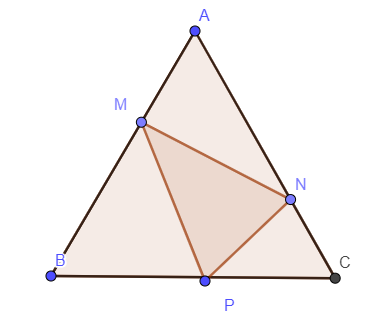
\includegraphics[width=0.3\linewidth]{anh1.png}
\end{figure}
\end{block}
\end{frame}


% 1.6 Phương pháp hình học
\begin{frame}{1.6 PHƯƠNG PHÁP HÌNH HỌC
\hspace{3cm}  70. Nguyễn Phương Thùy} 
%\framesubtitle{} 
\begin{block}{Giải:}
Dựng tam giác đều cạnh bằng một,$AM=x,PC=y,BN=z,$ như hình vẽ:\\Ta có :$S_{\Delta AMP} + S_{\Delta CPN} + S_{\Delta BMN} < S_{\Delta ABC} . $\\$ \Leftrightarrow \frac{1}{2}\sin{60^o}[x(1-y) + y(1-z) + z(1-x) ] < \frac{1}{2}\sin{60^o}.1.1.$\\ $\Leftrightarrow x(1-y) + y(1-z) + z(1-x) < 1.$(đpcm)

\begin{figure}
    \raggedleft
    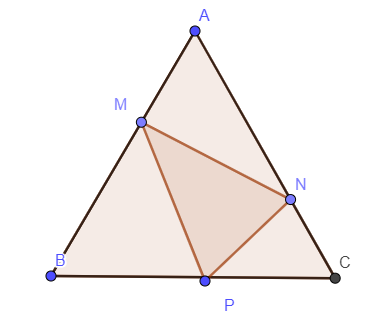
\includegraphics[width=0.25\linewidth]{anh1.png}
\end{figure}
\end{block}
\end{frame}

% 1.6 Phương pháp hình học
\begin{frame}{1.6 PHƯƠNG PHÁP HÌNH HỌC
\hspace{3cm}  70. Nguyễn Phương Thùy} 
%\framesubtitle{} 
\begin{block}{Bài toán 3:}
\textbf{Chứng minh bất đẳng thức Cauchy với hai số thực $a,b $ không âm.}\\
\end{block}
\end{frame}

% 1.6 Phương pháp hình học
\begin{frame}{1.6 PHƯƠNG PHÁP HÌNH HỌC
\hspace{3cm}  70. Nguyễn Phương Thùy} 
%\framesubtitle{} 
\begin{block}{Lời giải:}
\begin{figure}
    \centering
    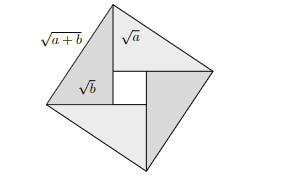
\includegraphics[width=0.7\linewidth]{anh2.png}
\end{figure}
\end{block}
\end{frame}


% 1.6 Phương pháp hình học
\begin{frame}{1.6 PHƯƠNG PHÁP HÌNH HỌC
\hspace{3cm}  70. Nguyễn Phương Thùy} 
%\framesubtitle{} 
\begin{block}{Lời giải:}\\Ta có : tổng diện tích của 4 tam giác vuông bên trong luôn bé hơn diện tích của hình vuông bao quanh có cạnh là $\sqrt{a+b}$,hay nói cách khác\\$(\sqrt{a+b})^2 \ge 4.\frac{1}{2}.\sqrt{a}.\sqrt{b} \Leftrightarrow a+b \ge \sqrt{ab} .$
\begin{figure}
    \raggedleft
    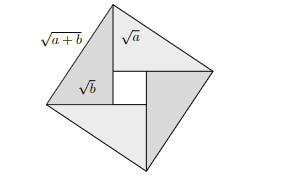
\includegraphics[width=0.5\linewidth]{anh2.png}
\end{figure}
\end{block}
\end{frame}




